
\section{Introduction}

Nb3Sn is a useful material for SRF cavities because it has a higher critical superconducting transition temperature (Tc) and superheating field (Hsh). Research on Nb3Sn SRF cavi-ties is motivated by their ability to achieve a high quality-factor, greater than 1010 at an operating temperature of 4 K, and high theoretical maximum accelerating gradient up to 100 MV/m. Despite the potential for higher accelerating gradients, Nb¬3Sn cavities have been limited to the 10-20 MV/m range with the highest performing cavities achieving 24 MV/m\cite{posen2021advances} The reason for this limited perfor-mance is thought to be due to imperfections formed during the manufacturing process of Nb3Sn cavities. 

Tin vapor-diffusion is the method of manufacturing Nb3Sn SRF cavities that has produced the highest perform-ing cavities to date. Niobium cavities are coated with a thin film of Nb3Sn through a tin-vapor reaction at elevated tem-peratures\cite{posen2021advances,pudasaini2019growth}. Nb3Sn grains nucleate and grow until the sur-face is completely covered. Once the surface is covered in an initial thin layer of Nb3Sn, the film continues to grow via tin diffusion through Nb3Sn grain boundaries (GBs)\cite{pudasaini2019growth}. 

The result is an imperfect film of Nb¬3Sn. Analysis of the film shows that it contains areas with low tin concentration known as tin-depleted regions\cite{lee2018atomic}. Depending on the coating parameters, the GBs may also be tin-rich or tin-deficient\cite{lee2020grain}. These stoichiometric differences can depress the critical su-perconducting transition temperature (Tc) of the material from 18 K down to as low as 6 K depending on the concen-tration of anti-site defects\cite{sitaraman2021effect}. A lower Tc causes an increase in the surface resistance of the cavity and makes it more likely to quench.

In addition to stoichiometric imperfections, the tin-vapor diffusion coated Nb3Sn films also have micro-scale surface roughness caused by faceting of the grains and thermal etch-ing at the grain boundaries. Surface roughness concentrates the magnetic field around sharp edges on the surface, there-by exceeding the critical field of the Nb3Sn prematurely\cite{porter2016surface}. The interface between the film and the niobium substrate is also uneven because of the interfacial reaction between nio-bium and tin\cite{lee2018atomic}. The film can become too thin in some areas, allowing the RF fields to interact with the niobium substrate and poorly superconducting Nb-Sn phases at the interface.

The 3-D structure of the Nb3Sn film becomes especially important when material is removed from the surface by polishing. Efforts have been made to polish Nb3Sn using electropolishing\cite{hu2019reducing}, buffered chemical polishing\cite{hu2019reducing}, and ox-ypolishing\cite{pudasaini2018studies}. These techniques remove material from the surface of the film, which could expose subsurface tin-deficient regions. Polishing is an important step for improv-ing the performance of niobium SRF cavities and will likely become an important step for Nb3Sn SRF cavity manufac-turing in the future. 

The structure of vapor diffusion coated Nb3Sn films has been studied by many people using transmission and scan-ning electron-microscopy (TEM and SEM)\cite{lee2018atomic,becker2015analysis,hall2017surface,hall2016surface}, and X-ray photo-emission spectroscopy (XPS)\cite{pudasaini2019growth,sun2019fast,hall2016surface}. These tech-niques provide 2-D or 1-D information about the chemical composition in the film and are therefore unable to deter-mine the 3-D distribution of tin-deficient regions. We can-not reliably determine how many of these regions are inter-acting with the RF fields, and we cannot determine their ef-fects on cavity performance using the currently available da-ta. 

In this study, we used a 3-D imaging method, focused ion-beam (FIB) tomography, to measure the distribution of tin inside vapor-diffusion coated Nb3Sn films to search for Sn-deficient regions and determine their impact on the per-formance of Nb3Sn vapor-diffusion coated cavities.

\section{Methodology}

\begin{figure}[htb]%
    \centering%
    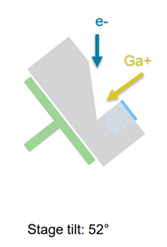
\includegraphics[width=0.25\columnwidth]{../figs/Figure-1.png}%
    \caption{}%
    \label{fig:1}%
\end{figure}


FIB tomography is a measurement technique that utilizes a combined FIB/SEM instrument. This facilitates rapid switching between electron beam imaging and ion beam milling. The ion beam is tilted \qty{52}{\degree} relative to the electron beam. During sample preparation and imaging, the stage is tilted \qty{52}{\degree} so that the ion beam is perpendicular to the sample's surface. A protective, \qty{2}{\micro\meter} thick Pt capping layer is deposited over the region-of-interest (ROI) to prevent damage from the ion beam over the course of the measurement. The sample is prepared by ion-beam milling a trench to expose a cross section of the sample surface. Then a clearance trench is milled on both sides of the ROI to ensure direct line-of-sight between the cross-section and the detector. This prevents shadows from forming in the electron beam image. Once the sample is prepared, the electron beam is employed to image the cross section. An automated process alternates between using the ion beam to mill a thin layer of material, creating a new cross section, and imaging each cross-section using the e-beam. The individual electron beam images are then combined to create a 3D image of the sample. A schematic of the beam and sample orientation is shown in figure~\ref{fig:1}

We employ energy dispersive X-ray spectroscopy (EDS) to measure the chemical composition of the sample. This method measures the emitted X-ray spectrum created by the e-beam when it is focused on a sample. Each element has a characteristic X-ray spectrum, which can be used to identify the chemical composition of the sample. To measure the distribution of tin in a sample, X-rays from the Sn L$\alpha$ X-ray series are counted. Regions of high tin concentration will emit more of these characteristic X-rays compared to low tin concentration regions.

We utilized a ThermoFischer Helios 5 FIB/SEM micro-scope to obtain the measurement. A \qty{30}{\kilo\volt}, \qty{2.7}{\nano\ampere} Ga+ ion-beam is employed to mill the sample. The electron-beam current and accelerating voltage are \qty{11}{\nano\ampere} and \qty{20}{\kilo\volt}. X-rays from the Sn L$\alpha$ series was counted by an Oxford Ultim® EDS detector. With these beam parameters, the EDS detec-tor was close to its maximum count rate of one million counts per second. The measured volume is approximately \qtyproduct[]{20 x 20 x 7}{\micro\meter}. The data was cropped to \qtyproduct[]{17 x 8 x 6}{\micro\meter} to re-move artifacts at the boundaries.  20 nm slices were cut for each e-beam image and the pixel size was 20x25.4 nm. The 3-D data set was binned and smoothed with a Gaussian fil-ter to minimize noise, yielding a final voxel size of 80x80x101.5 nm.

The sample is a 1cm diameter and \qty{4}{\milli\meter} thick niobium disk coated with a \qty{2}{\micro\meter} thick Nb3Sn film produced by the vapor-diffusion process\cite{pudasaini2019growth}. The samples were coated at \qty{1100}{\celsius} in a tin-coating furnace at Fermi National Accelera-tor Laboratory (FNAL). 

\section{Results}

Using the FIB tomography method, we were able to measure the 3-D distribution of tin inside a vapor-diffusion coated Nb3Sn film. This distribution is presented in figure~\ref{fig:2}, rendered using a volumetric shading technique. The surface of the film is visible, but it is difficult to observe the inter-nal structure of the film.
 
\begin{figure}[htb]%
    \centering%
    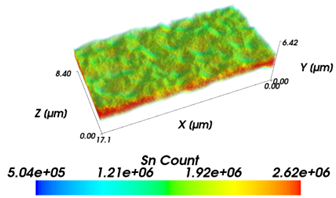
\includegraphics[width=0.5\columnwidth]{../figs/Figure-2.png}%
    \caption{}%
    \label{fig:2}%
\end{figure}

\begin{figure}[htb]%
    \centering%
    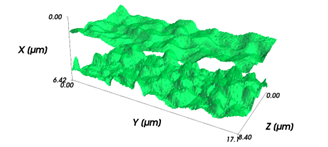
\includegraphics[width=0.5\columnwidth]{../figs/Figure-3.png}%
    \caption{}%
    \label{fig:3}%
\end{figure}

To better visualize the data, an isoconcentration surface is calculated. This surface intersects all the points in 3-D space with the same Sn X-ray signal intensity. From figure~\ref{fig:3} the surface roughness of the film can be observed, and the roughness of the Nb3Sn-Nb interface is also apparent.
 
The isosurface is used to calculate the thickness of the film by projecting a ray perpendicular to the X-Z plane and determining the distance between the intersec-tion points on the top and bottom surfaces of the Nb3Sn. From the thickness calculation, we calculate statistical parameters of the film such as the mean, minimum, and maximum thickness. The mean film thickness of the Nb3Sn film is \qty{2.0}{\micro\meter}, but some areas are as thin as \qty{0.7}{\micro\meter}. A map of the film thickness is displayed in figure~\ref{fig:4}

\begin{figure}[htb]%
    \centering%
    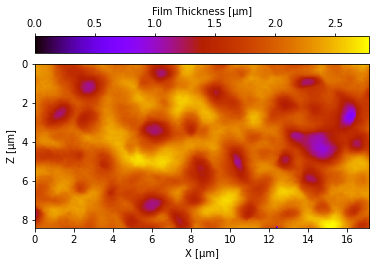
\includegraphics[width=0.5\columnwidth]{../figs/Figure-4a.png}%
    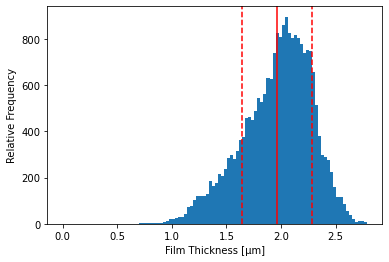
\includegraphics[width=0.5\columnwidth]{../figs/Figure-4b.png}%
    \caption{}%
    \label{fig:4}%
\end{figure}
 
To visualize the internal structure of the film, it is easier to analyze individual cross-sections of the data. Figure~\ref{fig:5} displays cross sections of the 3-D image at different locations in the film. These cross sections show several areas with low tin concentration including some areas that are within \qty{200}{\nano\meter} of the film surface. There is also a region where the thickness of the film decreases to less than \qty{1}{\micro\meter} due to a protrusion of the Nb substrate into the film.

\begin{figure}[htb]%
    \centering%
    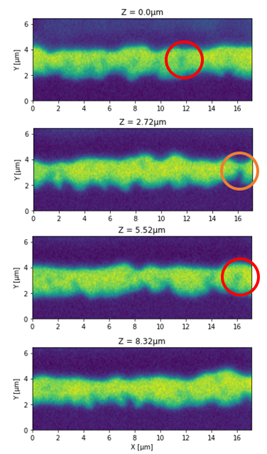
\includegraphics[width=0.5\columnwidth]{../figs/Figure-5.png}%
    \caption{}%
    \label{fig:5}%
\end{figure}

 
\section{Discussion}

Our results demonstrate that Sn-deficient regions and thin regions occur frequently near the surface of vapor-diffusion coated Nb3Sn films. We detected multiple regions where the Sn-concentration is less than the bulk Nb3Sn concentration, and we also found that the film is as thin as \qty{0.7}{\micro\meter} in some regions. This suggests that one cause of Nb3Sn SRF cavity performance degradation could be the interaction of the RF field with poorly superconducting, off-stoichiometric phases. However, it is difficult to estimate the magnitude of this effect compared to other sources of degradation such as surface roughness. Unless a tin-deficient region is located on the surface it will be shielded partially by the stoichiometric Nb3Sn. 

The effects of these near-surface imperfections are ex-pected to be more significant when applying a polishing treatment such as electropolishing, buffered chemical pol-ishing, or mechanical polishing, since these processes re-move the top layer of stoichiometric Nb3Sn and expose the imperfections, allowing them to interact more strongly with the RF field. 

We also find that the film has large fluctuations thick-ness. Therefore, polishing using chemical methods would quickly expose the underlying niobium substrate, since the Nb3Sn is as thin as \qty{0.7}{\micro\meter} in some areas. Exposing the niobium substrate would increase the surface resistance of the cavity and potentially expose poorly superconducting Nb-Sn phases that exist near the interface\cite{lee2018atomic}.

To remove the tin-deficient regions, changes may need to be made to the vapor diffusion coating parameters such as adjusting the temperature, coating duration, or changing the amount of tin vapor in the furnace to allow for tin diffusion into these off stoichiometry regions. For polished Nb3Sn films, the cavities could be reintroduced into the coating furnace to apply a new layer of tin to the surface which can react with the exposed tin-deficient regions and form a new layer of stoichiometric Nb3Sn on the surface.

The FIB Tomography method described in this paper also needs improvement. We would like to calculate statistical parameters about the size and distribution of the tin-depleted regions, but the contrast between the tin deficient regions and the bulk Nb3Sn is too low to programmatically distinguish the regions consistently. The low contrast of the image can be attributed to a low signal to noise ratio of the Sn X-ray signal and low spatial resolution.

The low spatial resolution is caused by the large interaction volume of the electron beam when using a high beam voltage, 20kV, and high beam current, 11nA. The X-rays are emitted from the entire interaction volume leading to blurring of the boundaries between areas of different chemical composition. Reducing the beam current and acceleration voltage will improve the spatial resolution and the sensitivity of the measurement to small changes in tin concentration. 

The signal-to-noise ratio of the measurement can also be improved by using the Nb L$\alpha$ X-ray signal to measure the local Nb-Sn ratio. The Nb L$\alpha$ X-rays have an energy of \qty{2.2}{\kilo\volt} compared to \qty{3.4}{\kilo\volt} for Sn L$\alpha$ X-rays\cite{osti_4794153}. This difference in energy leads to a 10 times greater X-ray intensity from niobium compared to tin. By incorporating both types of X-rays, the total X-ray count will be increased leading to a higher signal to noise ratio and lower acquisition times.


\section{Conclusion}

Using FIB tomography we found that Sn deficient regions and thin regions are a common feature of vapor diffusion coated Nb3Sn film. Additionally, we discovered that several of these regions are close to the surface of the film where they could interact with the RF field of the SRF cavity, especially if the film is chemically or mechanically polished. This suggests that subsurface tin deficient regions may play a role in degrading the performance of vapor diffusion coated Nb3Sn SRF cavities. Further research is required to quantify the effects of these subsurface imperfections on the performance of Nb3Sn SRF cavities. Methods of mitigating these regions, such as recoating the surface after polishing may need to be developed to achieve better performing SRF cavities. The FIB tomography meth-odology also needs to be optimized for imaging Nb3Sn films and tin deficient regions by improving the spatial res-olution and signal-to-noise ratio of the measurement.
